% !TEX root = Thesis.tex
\chapter{Layout Prototyping}\label{chap:prototyping}

  \begin{figure}[t]
    \centering
    \includegraphics[height=\textwidth]{Fig/proto_flow.eps}
    \caption{Flow of the proposed layout prototyping scheme.} 
    \label{fig:Proto_Flow}
  \end{figure}

  In this section, a prototyping flow is proposed as Figure~\ref{fig:Proto_Flow} illustrated. We first update the technology information for placement blocks and routing components. Later, the set of placement results are obtained by \textit{Multiple topologies generator} according to the extending DeFer in~\cite{ALP_YPWeng_iccad2011}. Multiple placement results which use the same hierarchical structure in Section~\ref{sec:HLE}. Mostly, the updated topologies of placement are changed. Once the placement topology is updated, the corresponding routing behavior should also be updated. The correlation between placement and routing is preserved as a crossing graph via CDT. Therefore, the crossing graph needs to be updated so that the routing can be reconnected correctly. Section~\ref{sec:updateG} represents the updating methodology, which further considers the routing direction changing in the migrated layout. The routing is generated on each of the placement candidate automatically by a bottom-up manner in Section~\ref{sec:GWRecon} and Section~\ref{sec:DRLegal}. 


  \section{Crossing Graph Updating}\label{sec:updateG}


    In order to obtain routing in the targeting placement with similar behavior to source layout, we update the crossing graph $G_{Cr}$ of each cluster into new placements which are generated from {\it Multiple Topologies Generator}. The overall {\it Crossing Graph Updating} procedure is represented in Algorithm~\ref{alg:CGU}. The objective motivation is to reflect the change of placement. Once the placement is changed, the coordinate of corners of blocks are changed as well. Since the locations of vertices are different from the original $G_{CDT}$, the updated graph $G'_{CDT}(V'_{CDT},E'_{CDT},B',T')$ is generated according to the new position/size of placement blocks. Figure~\ref{fig:CGU}(a) shows the original CDT graph $G_{CDT}$ of two placement blocks and Figure~\ref{fig:CGU}.(b) shows the changed graph $G'_{CDT}$. This graph has the same number of vertices, edges, triangles, and blocks with $G_{CDT}$, but with different vertex coordinates. $G'_{CDT}$ is no longer a CDT graph since its edges and triangles are distorted from the original one. (It is like the original graph being stretched.) Some edges might overlap with placement blocks, which are represented as solid blue line in Figure~\ref{fig:CGU}(b).

    \newcommand{\CGU}{\ensuremath{\mbox{\sc CrossGraphUpdate}}}
    \begin{algorithm}[t]  
      \caption{$\CGU(G_{Cr},B',V_{RP}')$}\label{alg:CGU}                       
      \begin{scriptsize}
        \begin{algorithmic}[1]
          \REQUIRE 
            \begin{tabular}{l}
              $G_{Cr}(V_{CDT}\cup V_{Cr}, E_{CDT} \cup E_{Cr},B,T)$: The original crossing graph\\
              $B'$: The set of placement blocks with updated coordination \\
              $V_{RP}'$ Updated corners of layout and the middle-points of each plane boundary
            \end{tabular}
          \ENSURE 
            \begin{tabular}{l}
              $G_{Cr}'(V_{CDT}'\cup V_{Cr}',E_{CDT}'\cup E_{Cr}',B',T')$
            \end{tabular}
          \STATE $(E_{CDT}',T',E_{Cr}',V_{Cr}') \gets UpdateCoordinate(E_{CDT},T,E_{Cr},V_{Cr})$
          \FOR {$i = 1 \to |E_{CDT}|$}
            \IF {$InValid({e_{CDT}}_i,B')$}\label{line:CEUstart}
              \STATE $E_{CDT}' \gets E_{CDT}' - {e_{CDT}}_i'$
              \STATE $T' \gets T' - AdjacentTriangles({e_{CDT}}_i)$
              \IF {${e_{CDT}}_i' \in E_{Cr}$}
                \STATE $E_{Cr}' = E_{Cr}'- {e_{CDT}}_i'$
                \STATE $V_{Cr}' = V_{Cr}'- GetCrossVertices({e_{CDT}}_i')$
              \ENDIF\label{line:CEUend}
            \ELSE\label{line:RefDirUstart}
              \STATE $v_{Cr}' \gets CrossPoints({e_{CDT}}'_i)$
              \STATE $\overrightarrow{E_x} + \overrightarrow{E_y} = \overrightarrow{{e_{CDT}}_i}$
              \STATE $\overrightarrow{E_x}' + \overrightarrow{E_y}' = \overrightarrow{{e_{CDT}}_i}'$ 
              \FOR {$j = 1 \to |v_{Cr}'|$}
                \IF { $|\overrightarrow{E_x}' - \overrightarrow{E_x}|= |\overrightarrow{E_x}'|+|\overrightarrow{E_x}| \wedge GetRefDir(v_{Cr}^j)=V$ }
                  \STATE $RefDir({v_{Cr}^j}')\gets H$
                \ELSIF {$|\overrightarrow{E_y}' - \overrightarrow{E_y}|= |\overrightarrow{E_y}'|+|\overrightarrow{E_y}| \wedge GetRefDir(v_{Cr}^j)=H$ }
                  \STATE $RefDir({v_{Cr}^j}') \gets V$
                \ENDIF
              \ENDFOR
            \ENDIF\label{line:RefDirUend}
          \ENDFOR
          \RETURN $G_{Cr}'(V_{CDT}'\cup V_{Cr}',E_{CDT}'\cup E_{Cr}',B',T')$
        \end{algorithmic}
      \end{scriptsize} 
    \end{algorithm}

    \begin{figure}[ht]
      \begin{center}
      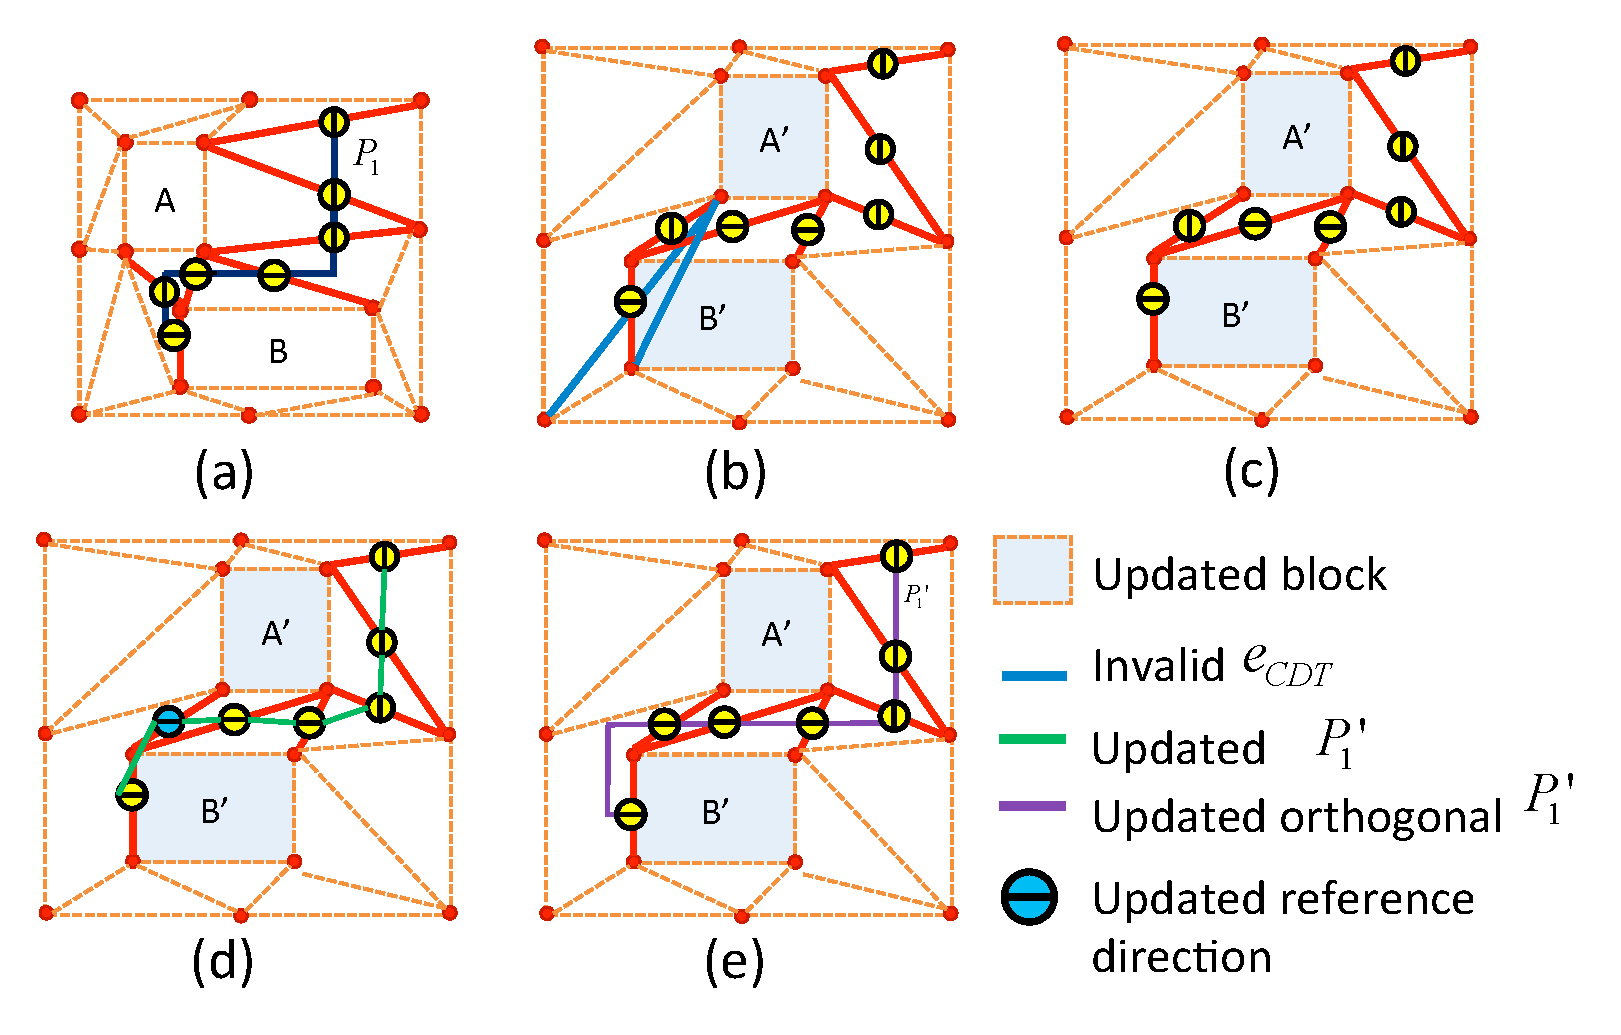
\includegraphics[width=\textwidth]{Fig/UCG.eps}
      \caption{
        Updating crossing graph to reflect placement change.
        (a) Illustration of the original crossing graph.
        (b) A crossing graph with updated $V_{CDT}'$ with different coordinates. 2 blue solid lines as invalid $e_{CDT}'$ since they overlap with block $B'$.
        (c) Removing invalid $e_{CDT}'$.
        (d) Changing reference direction of a crossing point and reconnecting $P_1'$ among $V_{Cr}'$. 
        (e) Reconstructing $P_1'$ by orthogonal segments.
      }
      \label{fig:CGU}
      \end{center}
    \end{figure}


    Notice that once an edge overlaps with blocks in graph $G'_{CDT}$, it actually reveals the correlation vanished between placement blocks, 
    which means the edge no longer represents a routing channel.
    These overlapping edges are set to be {\it invalid} to indicate that the routing information stored on this edge is incorrect.
    According to Figure~\ref{fig:CGU}.(c), the crossing graph $G_{Cr}$ is updated by removing the invalid crossing edges and the invalid crossing point on them. The detail updating process is described in Algorithm~\ref{alg:CGU} from line~\ref{line:CEUstart} to line~\ref{line:CEUend}.
    On the contrary, if there does not exist any overlapping between edges and blocks in $G'_{CDT}$, the routing behavior can be well preserved even if the layout changes.

      

    \begin{figure}[t]
      \begin{center}
        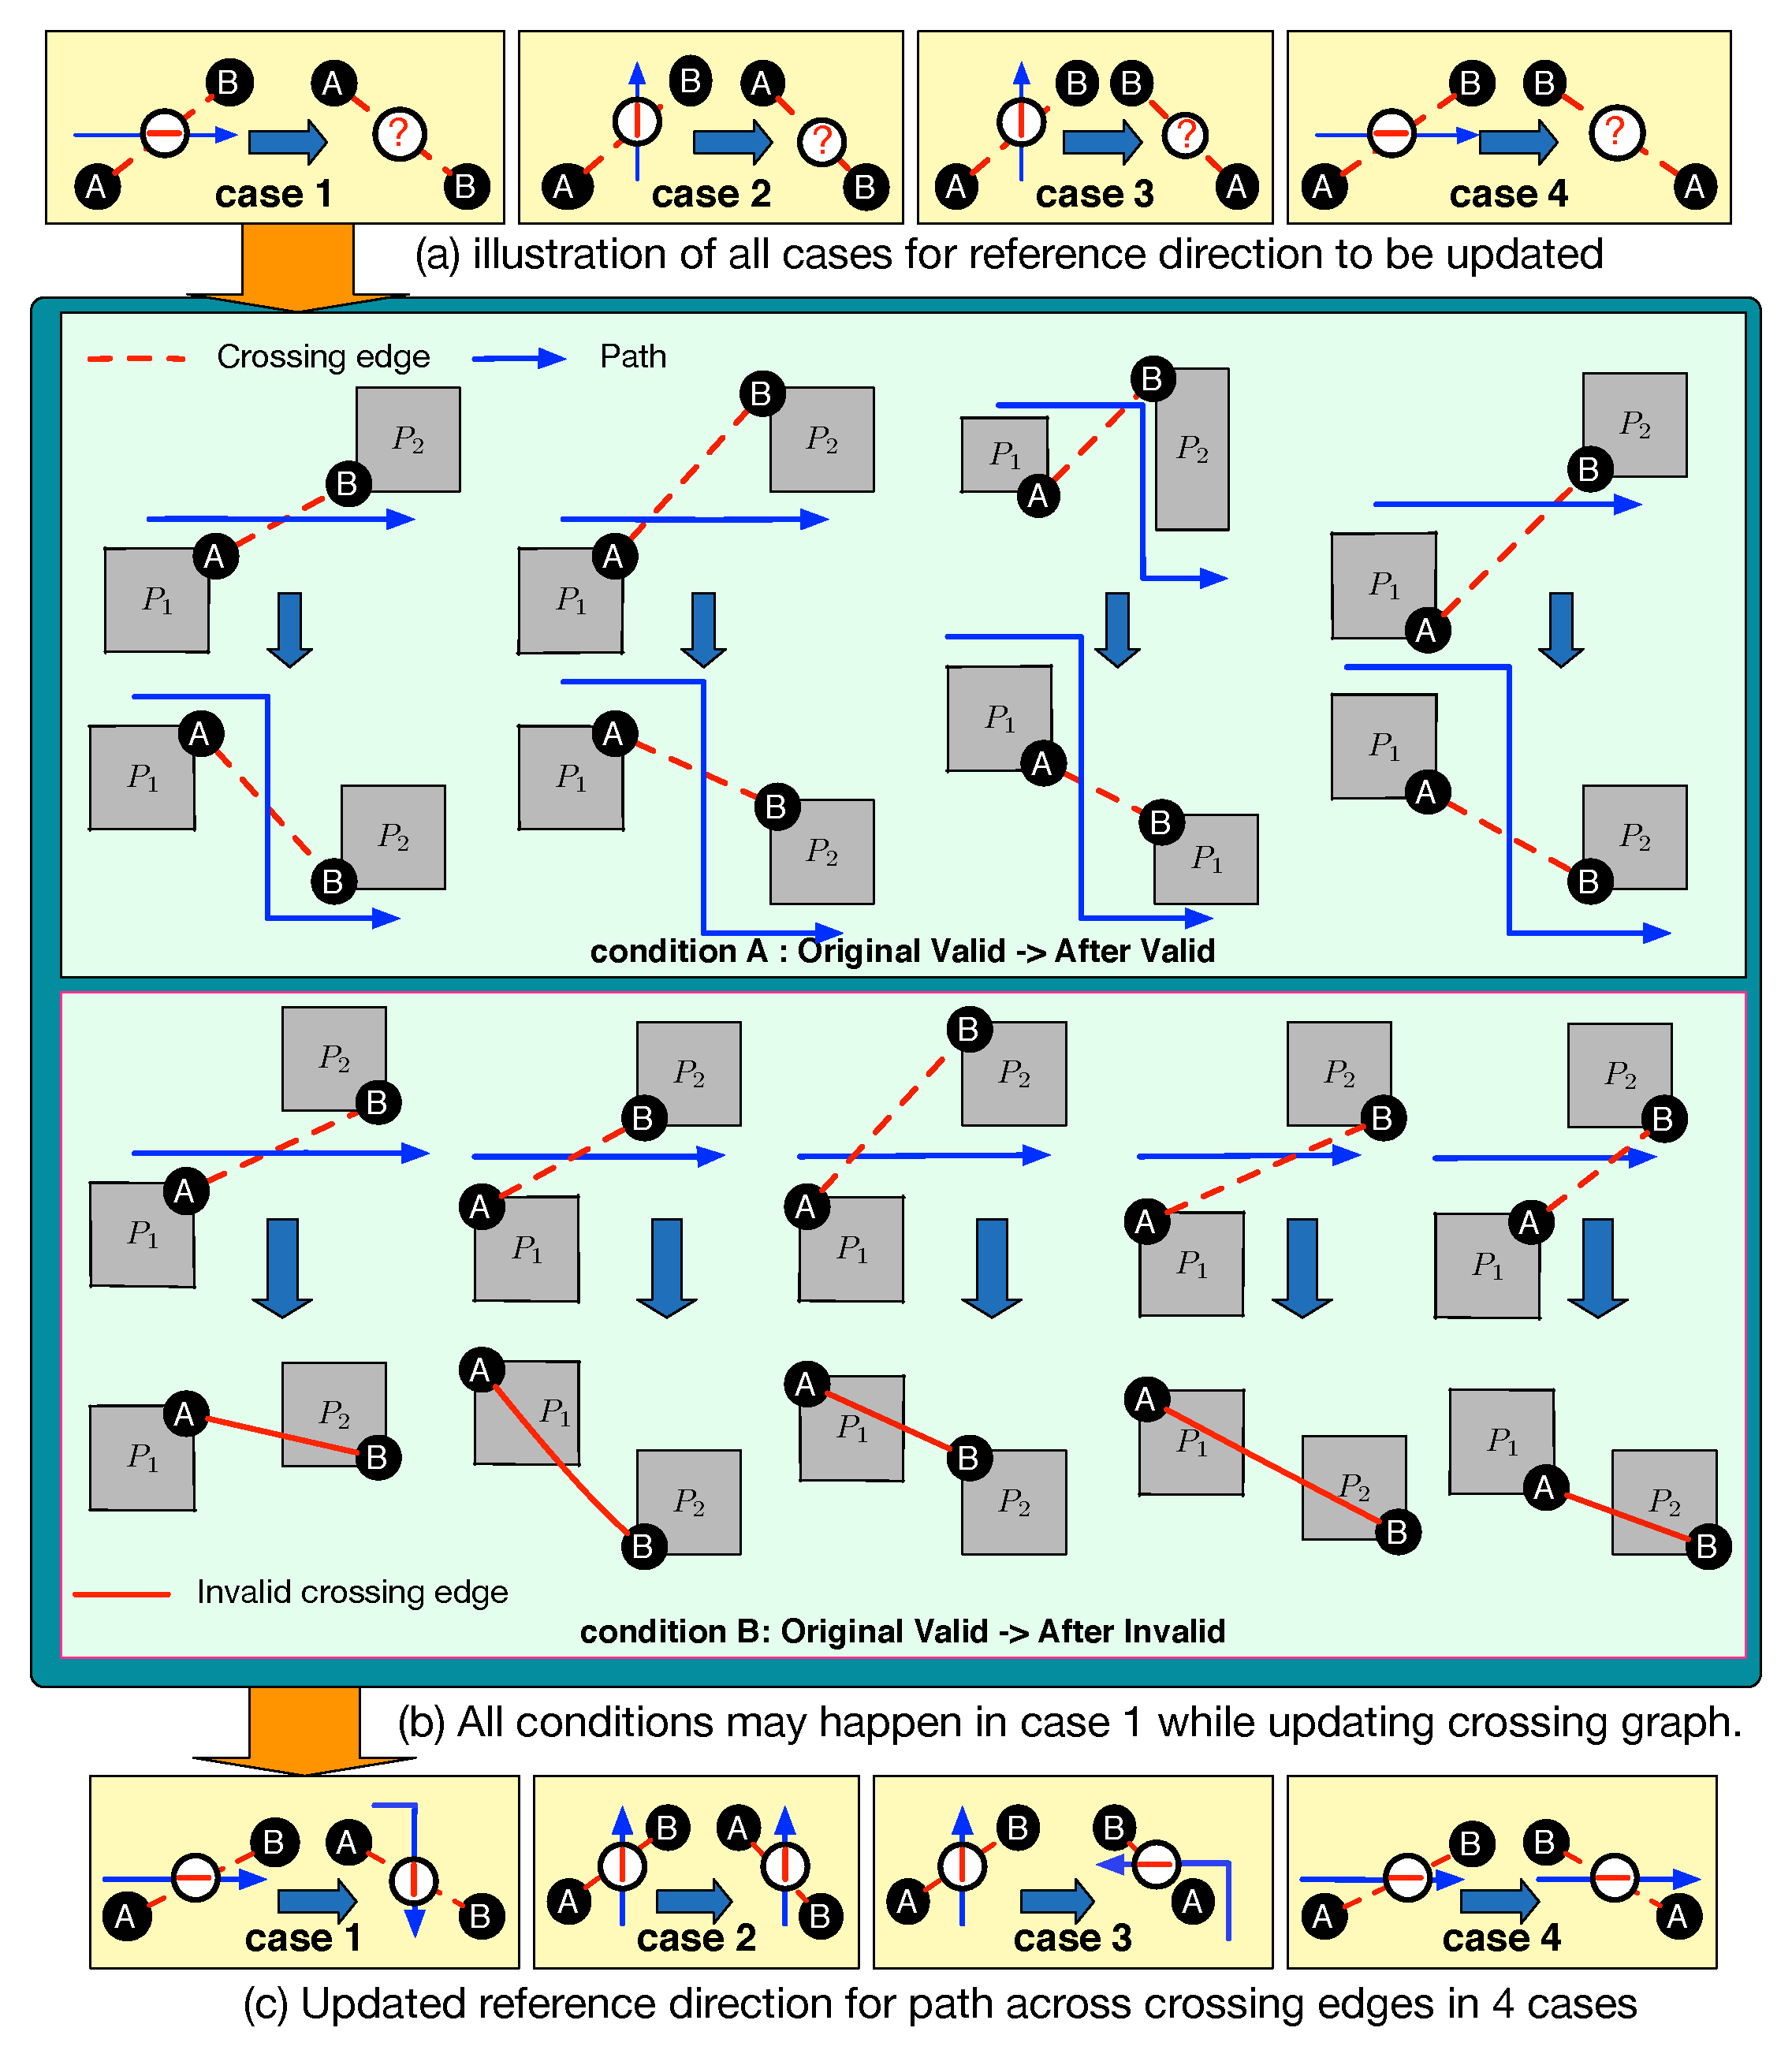
\includegraphics[width=\textwidth]{Fig/dirch.eps}
        \caption{4 cases of updating reference direction for routing path while crossing edge $\protect\overrightarrow{AB}$ changes.}
        \label{fig:dirch}
      \end{center}
    \end{figure}

    The reference directions stored on crossing points give a superb hint when reconstructing routing paths on a different placement.
    In certain cases, the direction should be changed from H to V (or V to H) due to the slope of CDT edge varies. As illustrated in Figure~\ref{fig:CGU}.(d), there are seven crossing points, three of them have direction V and the others have direction H. However, the direction of the blue crossing points cannot be vertical due to the x direction vector of the corresponding CDT edge changed from negative to positive. If such situation occurs, the reference direction will be changed from V to H. We further discuss the conditions that are supposed to happen while updating crossing edge.

     
    One path is given across the channel between $\overline{AB}$ in vertical or horizontal. As illustrated in Figure~\ref{fig:dirch}.(a), there are 4 cases that may occur when updating the crossing graph. If one crossing edge $\overline{AB}$ connects two blocks $P_1$ and $P_2$, A is one of the corners on $P_1$ and B is one of the corners on $P_2$. Since each of $P_1$ and $P_2$ has four corners, there are at most 16 ($4\times 4$) combinations to form $\overline{AB}$. However, there are 7 combinations that the crossing edges initially overlap with $P_1$ or $P_2$. In Figure~\ref{fig:dirch}.(a), we consider the crossing edge $\overline{AB}$ as a vector $\overrightarrow{AB}$. In case 1, if the y-direction vector changes conversely, all the possible 9 results of case 1 is shown in Fig~\ref{fig:dirch}.(b). These results can be categorized into two conditions as follows,
    \begin{itemize}
      \item{\bf Condition A: Origin-Valid-After-Valid}, the crossing edge $\overrightarrow{AB}$ is originally valid and it keeps valid after the crossing graph updated. To keep the path above block $P_1$ and below $P_2$, the path changes it direction from horizontal to vertical while crossing $\overrightarrow{AB}$.
      \item{\bf Condition B: Origin-Valid-After-Invalid}, the crossing edge is invalid after updating crossing graph. In other words, the relationship is broken.
    \end{itemize}

    \begin{figure}[t]
      \begin{center}
        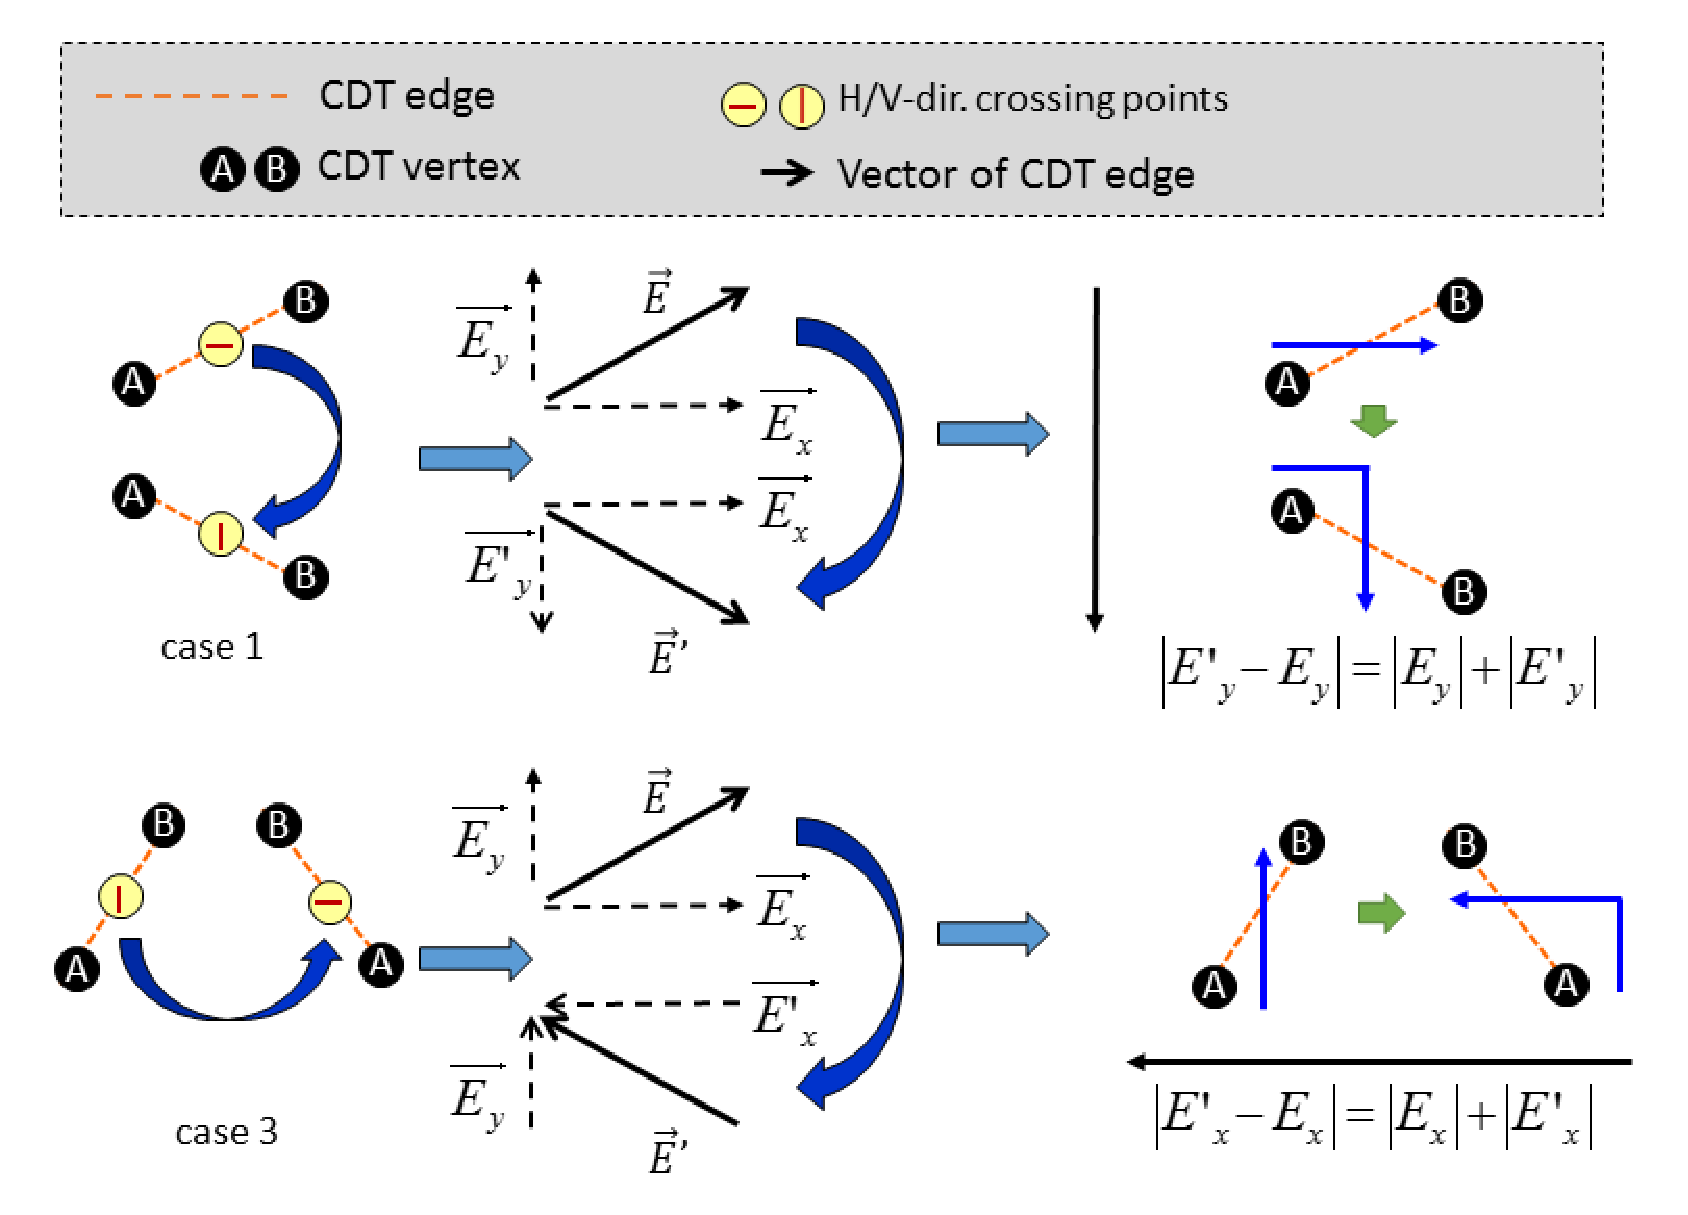
\includegraphics[width=\textwidth]{Fig/refdir3.eps}
        \caption{Reference direction updating due to angle changing of CDT edge.
         In case 1, H-direction crossing points are updated to V. 
           In case 3, V-direction crossing points are updated to H.}
        \label{fig:refdir}
      \end{center}
    \end{figure}

    Therefore, the reference direction of the path in case 1 is updated from horizontal (H) to vertical (V) after updating crossing graph. Likewise, if the x-direction vector changes conversely as case 3 in Figure~\ref{fig:dirch}.(a) illustrated, the reference direction should be change to horizontal (H). The rest case 2 and case 4 keep the same reference direction while updating crossing graph. Figure~\ref{fig:dirch}.(c) reveals the reference direction of the routing path after updating crossing graph in the above cases.

    The situation is generalized into two cases as listed in Figure~\ref{fig:refdir}.
    For a CDT edge $E$, assume the two endpoints are vertex A and vertex B. Without loss of generality, we consider edge E as a vector $\overrightarrow{E}$, which can be decomposed into x-direction vector $\overrightarrow{E_x}$ and y-direction vector $\overrightarrow{E_y}$. According to Figure~\ref{fig:refdir}, case 1 and 3 from Figure~\ref{fig:dirch} are demonstrated for reference direction changing as follow, 

    


    \begin{enumerate}
      \item For a case that the difference of y-direction vector between $\overrightarrow{E}$ and $\overrightarrow{E'}$ equals the sum of both y-direction vectors' modulus, where $|\overrightarrow{E_y'} - \overrightarrow{E_y}|=|\overrightarrow{E_y'}|+|\overrightarrow{E_y}|$. It indicates that the vertical direction of the updated CDT edge is opposite to the origin. Therefore, if the reference direction of the crossing edge is horizontal primitively, it should be updated to vertical for path extension.
      \item For a case that the difference of x-direction vector between $\overrightarrow{E}$ and $\overrightarrow{E'}$ equals the sum of both x-direction vectors' modulus, where $|\overrightarrow{E_x'} - \overrightarrow{E_x}|=|\overrightarrow{E_x'}|+|\overrightarrow{E_x}|$. It indicates that the horizontal direction of the updated CDT edge is opposite to the origin. Therefore, if the reference direction of the crossing edge is vertical primitively, it should be updated to horizontal for path extension.
    \end{enumerate}

    

    With this process from line~\ref{line:RefDirUstart} to line~\ref{line:RefDirUend} in Algorithm~\ref{alg:CGU}, the reference directions can be correctly updated.

    

  \section{Global Wire Reconstruction By Orthogonal Segments}\label{sec:GWRecon}
    For each cluster $i$ of input design, we re-construct routing paths according to the corresponding crossing graph $G_{Cri}$.
    Recall that each crossing point $v \in V_{Cr}$ in $G_{Cri}$ is with a reference direction stored on it.
    For each $G_{Cri}$, the orthogonal wire segments are generated as follows:
    (a) adjacent crossing points with the same reference direction are aligned to produce a set of vertical/horizontal segments.
    (b) if step (a) does not produce illegal routing such as crossing with other modules/devices, it will be preserved, else
    (c) the program will split the segment into several sub-segments with each sub-segment can be routed using the reference direction legally, and then we connect these sub-segments using pattern route.
    (d) wire spacing constraint of each metal layer are examined and adjusted by shifting segments.


  \section{Detailed Routing Legalization}\label{sec:DRLegal}
    Once the routing reconnection of all bottom level clusters are complete, 
    these clusters are regarded as placement blocks in the upper level,
    and the wire segments connected to the block boundary are taken as pin locations in the upper level.
    The procedure is repeated until the top-level design of routing is obtained.

  Since all the above steps are implemented automatically, each net still needs to be patched in detail. For instance, the pin connections inside the devices are done manually since the location inside each devices are changed from the source layout to the target technology. 
  However, since we perform detailed routing legalization scheme in a comprehensive view, most of the tasks are covered and the detail refinement is easier to implement for analog layout designers.
  
  Note that the routing behaviors are generally preserved in the targeting layout due to the similarity among the original placement and the targeting placement. Thus, the preservation of routing is flexible. The fundamental idea of routing preservation in this paper is to preserve the corresponding wires with the placement topology. If the designers decide to select a different placement topology, the necessity of preservation for routing is less. Hence, that is what our triangulation-based preservation provides.


